\chapter{Einleitung}

Einleitung beginnt hier. 
Hier ein Beispiel eines Zitats:
\begin{quote}
According to all known laws
of aviation,

there is no way a bee
should be able to fly.

Its wings are too small to get
its fat little body off the ground.
\footnote{
Simon Smith und Steve Hickner, 
url: \url{http://www.script-o-rama.com/movie_scripts/a1/bee-movie-script-transcript-seinfeld.html}, 
Abrufdatum: 2022-02-18\cite{bee_movie}
}
\end{quote}
\vspace{-0.5cm} % negative vertical spacing
\begin{flushright}
{\footnotesize Note: Not true.} 
\end{flushright}

Anführungszeichen können durch den Befehl \textbackslash{}enquote \enquote{verwendet} werden, da es an den Sprach-Style angepasst werden kann und "das" nicht korrekt dargestellt wird.
Sonderzeichen wie z. B. Unterstriche müssen aber gesondert behandelt werden \enquote{ein\_wort}.

Beispiele für mathematische Formeln:
\begin{enumerate}
    \item $\mathbf{Q} = \{{\frac{a}{b}} \mid a,b \in \mathbf{Z} , b \neq 0\}
        \Rightarrow |\mathbf{Q}| \leq 1$
    \item $(x \neq 0 \; \land \; (y = 0 \; \lor \; x < y))$
    \item $\sim150$
\end{enumerate}

\clearpage % Page-Break

Eine nicht-nummerierte Liste:
\begin{itemize}
    % reduce spacing between items
    \setlength{\itemsep}{5pt}
    \setlength{\parskip}{0pt}
    \setlength{\parsep}{0pt}
    %
    \item The bee, of course, flies anyway
    \item because bees don't care what humans think is impossible.
    \item Yellow, black. Yellow, black. Yellow, black. Yellow, black.
    \item Ooh, black and yellow! Let's shake it up a little.
\end{itemize}


\section{Problembeschreibung}

Hier kann z.B. das Problem erläutert werden, aus welchem die Thesis entstanden ist.

Lorem ipsum dolor sit amet, consectetur adipiscing elit. Integer efficitur ipsum ut nulla dignissim tincidunt. Nullam sit amet tempor urna. Ut euismod mattis orci, vel mattis mi malesuada in. Aliquam molestie fermentum vestibulum. Cras egestas molestie ipsum, vitae malesuada ante consectetur id. In turpis neque, pharetra eget neque vel, rhoncus tincidunt ex. Sed lacinia fermentum odio quis faucibus. Phasellus blandit orci vitae ipsum rutrum aliquam. Fusce ipsum nisl, luctus in interdum non, sodales sed lacus. Fusce vitae fermentum tellus, vitae feugiat magna. Curabitur tincidunt mauris ac venenatis accumsan. Mauris efficitur sit amet mauris in sodales. Ut fringilla commodo sem, at commodo erat mattis sed.

Integer venenatis convallis erat, sit amet elementum odio egestas interdum. Phasellus sagittis vestibulum libero vel sodales. Phasellus a facilisis felis, vel mollis velit. Quisque pulvinar turpis vitae bibendum condimentum. Nulla facilisi. Praesent iaculis euismod eros et consequat. Nullam efficitur facilisis sapien. Aenean non laoreet lectus. Phasellus tellus lorem, ullamcorper vel aliquam ut, sollicitudin accumsan nibh. Duis vel elementum justo. Proin sed enim ipsum. Morbi sed mattis neque. Nulla varius dui a purus tempor elementum. Donec at nisl tortor. Pellentesque consequat porta aliquet. 

\clearpage

\begin{figure}[ht]
    \centering
    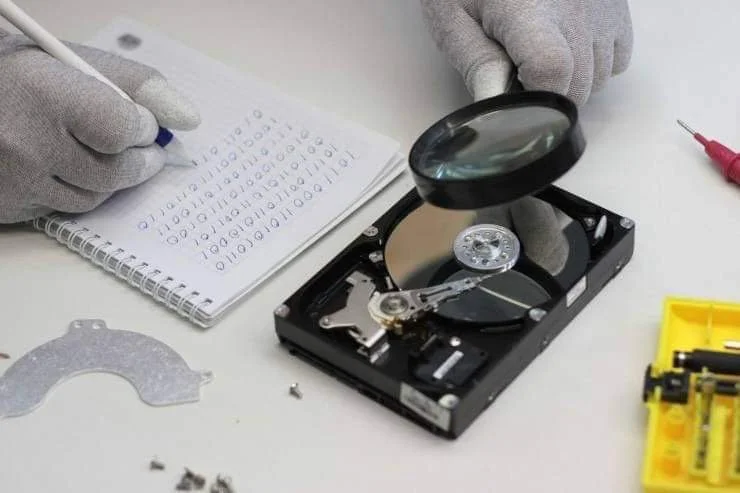
\includegraphics[width=0.8\textwidth]{bilder/read_hard_drive.png} % 80% der Textbreite
    \caption
    [Auslesen einer Festplatte] % Text, der im Bildverzeichnis verwendet wird
    {Auslesen einer Festplatte\cite{quelle}} % citation in der Beschriftung aber nicht im Bildverzeichnis
    \label{fig:old_db}
\end{figure}

\begin{wraptable}[9]{r}{8cm} 
% [9] = Höhe von neun Zeilen, {r} = rechts, {8cm} = Breite von 8cm (0.6\textwidth geht z.B. auch)
\begin{center}
\begin{tabular}{||c c c||} 
    \hline
    Name & anderer Name & eine Anzahl \\ [0.5ex] 
    \hline\hline
    Joanne &
    Esparza &
    $\sim$ 35 \\
    \hline
    Ivor &
    Sullivan &
    $\sim$ 82 \\ 
    \hline
    Martin & 
    Southern &
    $\sim$ 35 \\
    \hline
    Karina & 
    Willis &
    $\sim$ 32 \\
    \hline
\end{tabular}
\end{center}
\caption{Anzahl Einträge in den Tabellen}
\label{tab:bsp_tabelle}
\end{wraptable} 

Hier noch eine Grundlegende Tabelle, die neben dem Text steht.
Die Tabelle \ref{tab:bsp_tabelle} kann durch das Label referenziert werden.
Auf gleiche Weise können auch Kapitel, Bilder, etc. referenziert werden.

Lorem ipsum dolor sit amet, consectetur adipiscing elit. Integer efficitur ipsum ut nulla dignissim tincidunt. Nullam sit amet tempor urna. Ut euismod mattis orci, vel mattis mi malesuada in. Aliquam molestie fermentum vestibulum. 

Cras egestas molestie ipsum, vitae malesuada ante consectetur id. In turpis neque, pharetra eget neque vel, rhoncus tincidunt ex. Sed lacinia fermentum odio quis faucibus. Phasellus blandit orci vitae ipsum rutrum aliquam. Fusce ipsum nisl, luctus in interdum non, sodales sed lacus. 


\clearpage

\section{Überblick}
\label{kap:ueberblick}

Hier kann ein Überblick über folgenden Kapitel dargestellt werden.

Lorem ipsum dolor sit amet, consectetur adipiscing elit. Integer efficitur ipsum ut nulla dignissim tincidunt. Nullam sit amet tempor urna. Ut euismod mattis orci, vel mattis mi malesuada in.

In turpis neque, pharetra eget neque vel, rhoncus tincidunt ex. Sed lacinia fermentum odio quis faucibus. 

Phasellus blandit orci vitae ipsum rutrum aliquam. Fusce ipsum nisl, luctus in interdum non, sodales sed lacus. Fusce vitae fermentum tellus, vitae feugiat magna. Curabitur tincidunt mauris ac venenatis accumsan. 